\begin{frame}[allowframebreaks]{Cycle GANs}

\begin{itemize}
    \item Unpaired Image-to-Image Translation using Cycle-Consistent Adversarial Networks, Efros, ICC7 2017
    
\end{itemize}
\begin{figure}
    \centering
    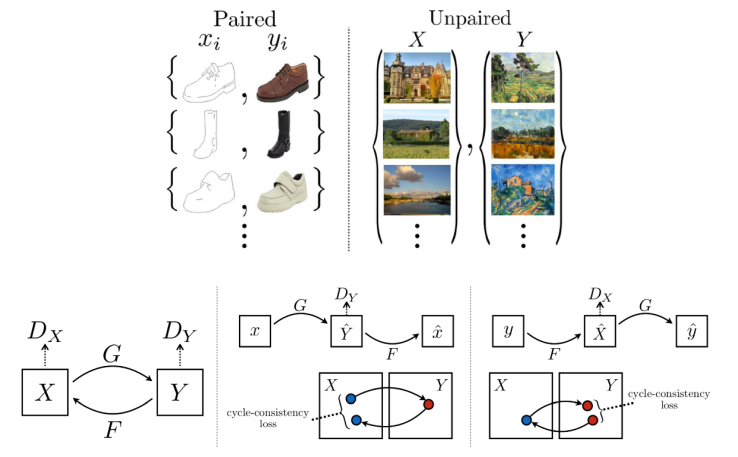
\includegraphics[height=0.7\textheight, width=\textwidth, keepaspectratio]{images/gan/cycle_gan_1.png}
\end{figure}
\framebreak
$$C_{horse \rightarrow zebra} = horse \rightarrow G_{horse \rightarrow zebra} \rightarrow \hat{zebra} \rightarrow [D_{zebra}, G_{zebra \rightarrow horse}] \rightarrow \hat{horse}$$
\begin{figure}
    \centering
    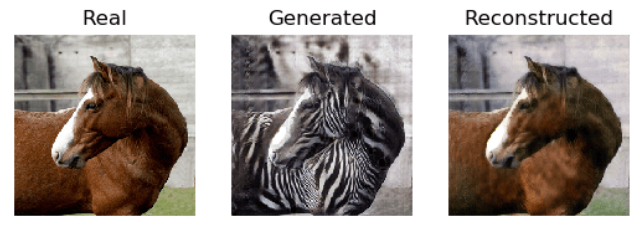
\includegraphics[height=0.7\textheight, width=\textwidth, keepaspectratio]{images/gan/cycle_gan_2.png}
\end{figure}

\framebreak
$$C_{zebra \rightarrow horse} = zebra \rightarrow G_{zebra \rightarrow horse} \rightarrow \hat{horse} \rightarrow [D_{horse}, G_{horse \rightarrow zebra}] \rightarrow \hat{zebra}$$
\begin{figure}
    \centering
    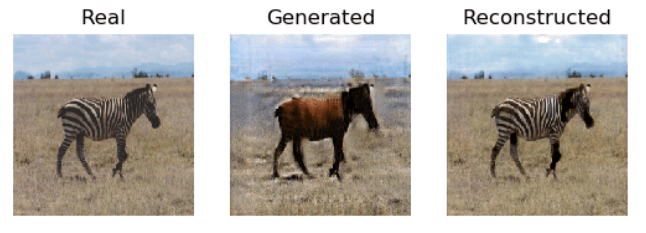
\includegraphics[height=0.7\textheight, width=\textwidth, keepaspectratio]{images/gan/cycle_gan_3.png}
\end{figure}

\framebreak
\begin{figure}
    \centering
    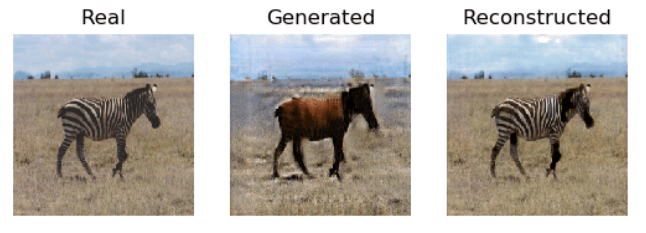
\includegraphics[height=0.7\textheight, width=\textwidth, keepaspectratio]{images/gan/cycle_gan_3.png}
\end{figure}

\framebreak
\begin{figure}
    \centering
    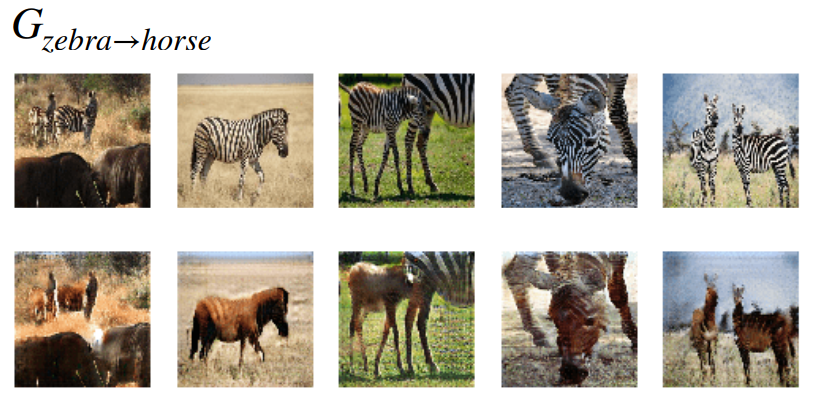
\includegraphics[height=0.9\textheight, width=\textwidth, keepaspectratio]{images/gan/cycle_gan_4.png}
\end{figure}

\framebreak
\begin{figure}
    \centering
    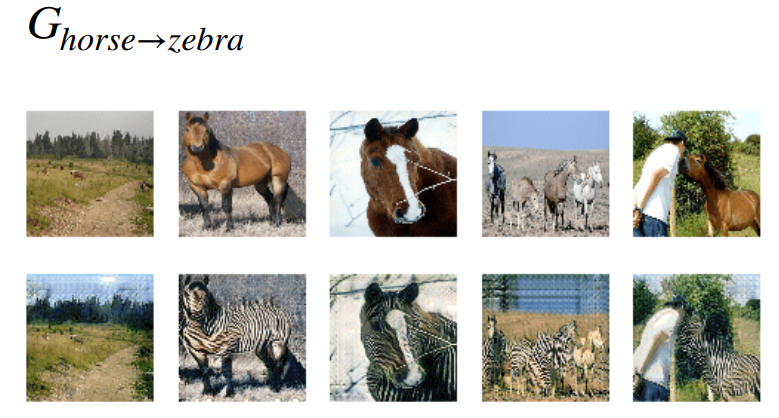
\includegraphics[height=0.9\textheight, width=\textwidth, keepaspectratio]{images/gan/cycle_gan_5.png}
\end{figure}

\framebreak
\begin{figure}
    \centering
    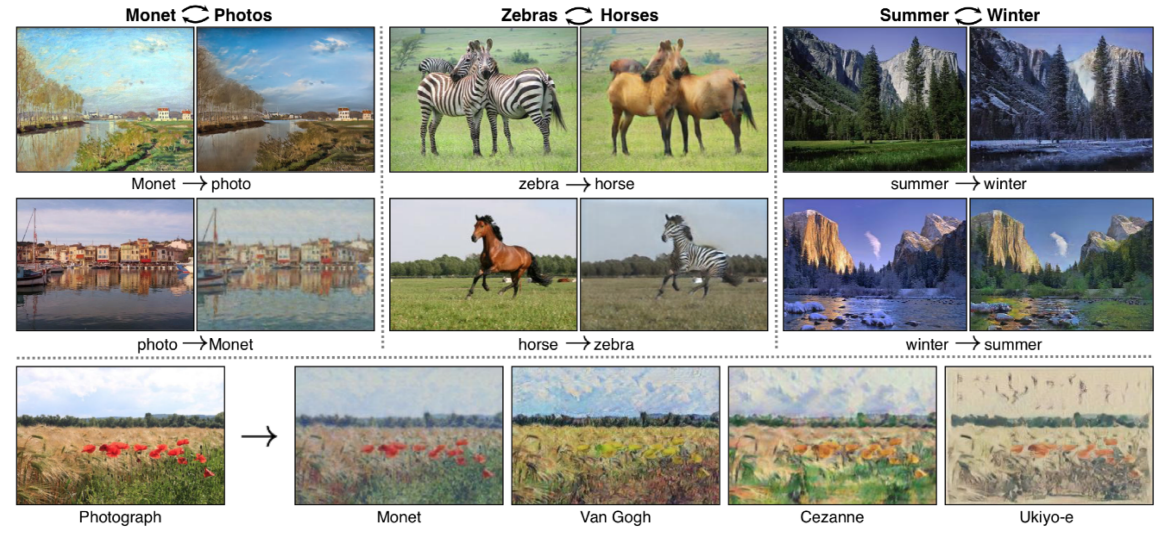
\includegraphics[height=0.9\textheight, width=\textwidth, keepaspectratio]{images/gan/cycle_gan_6.png}
    \caption{Image to Image translation with Cycle GANs}
\end{figure}
\end{frame}